\documentclass{article}
\usepackage{../../fasy-hw}

\title{Computational Geometry, Homework \hwnum}
\collab{n/a}

%% Instructor: update these macros:
\renewcommand{\hwnum}{1}
\date{due: 23 February 2023}

%% Student: update this macro:
\author{\todo{Your Name Here}}

\begin{document}

\maketitle

This homework assignment should be
submitted as a single PDF file to D2L.

General homework expectations:
\begin{itemize}
    \item Homework should be typeset using LaTex.
    \item Answers should be in complete sentences and proofread so that they
        make sense without seeing the question.
    \item You will not plagiarize, nor will you share your written solutions
        with classmates. (But, discussing the questions is highly encouraged).
    \item List collaborators at the start of each question using the
        \texttt{collab} command.
    \item Put your answers where the \texttt{todo} command currently is (and
        remove the \texttt{todo} macro, but not the word \texttt{Answer}).
    \item If you are asked to come up with an algorithm, you are
        expected to give an efficient algorithm (brute-force solutions will not
        be accepted). With your algorithm, please provide the following:
        \begin{itemize}
            \item \emph{What}: A prose explanation of the problem and the algorithm,
                including a description of the input/output.  Be sure to state
                your GP assumptions.
            \item \emph{How}: Describe how the algorithm works clearly.
                Including pseudocode may helpful.
            \item \emph{How Fast}: Runtime, along with the derivation.  (Or, at
                the very least, a proof of termination using a decrementing
                function).  You only need to specify the space complexity if the
                problem asks for it.
           \item \emph{Why}: Brief justification of why the algorithm works.
               Often, this will include a statement of the loop invariant for each
               (outer-most) loop, or recursion invariant for each recursive function.
        \end{itemize}
\end{itemize}

{\bf David Mount's tips for writing up homework solutions}:
Remember that your description is intended to be read by a
human, not a compiler, so conciseness and clarity are preferred over technical
details.  Unless otherwise stated, you may use any results from class, or
results from any standard textbook on algorithms and data structures. Also, you
may use results from geometry that: (1) have been mentioned in class, (2) would
be known to someone who knows basic geometry or linear algebra, or (3) is
intuitively obvious. If you are unsure, please feel free to check with me.

Giving careful and rigorous proofs can be quite cumbersome in geometry, and so
you are encouraged to use intuition and give illustrations whenever appropriate.
Beware, however, that a poorly drawn figure can make certain erroneous
hypotheses appear to be ``obviously correct.''

Throughout the semester, unless otherwise stated, you may assume that input
objects are in general position. For example, you may assume that no two points
have the same x-coordinate, no three points are collinear, no four points are
co-circular. Also, unless otherwise stated, you may assume that any geometric
primitive involving a constant number of objects each of constant complexity can
be computed in $\Theta(1)$ time


{\bf Acknowledgement}: the homework problems were adapted from assignments of David
Millman, which, in turn, were adaptations of problems by David Mount and Carola
Wenk.

%%%%%%%%%%%%%%%%%%%%%%%%%%%%%%%%%%%%%%%%%%%%%%%%%%%%%%%%%%%%%%%%%%%%%%%%%%%%%%
\collab{\todo{}}
\nextprob{Short Answers}

Provide short answers to the following questions

\begin{enumerate}
    \item What is the difference between best-case analysis and $\Omega$
        notation?

        \paragraph{Answer}
        \todo{replace this TODO with your answer}

    \item Choose a problem in the
        \href{https://www3.cs.stonybrook.edu/~algorith/major_section/1.6.shtml}{Stony Brook Algorithm
        Repository},
        describe the problem in your own words, and find somewhere that this
        technique (or something close to it) is or can be used.  Be sure to
        include proper citations (of a research paper or newspaper article, or
        whatever source you use).

        \paragraph{Answer}
        \todo{replace this TODO with your answer}

    \item The next three questions are about the DCEL data structure.  Let
        $\vec{e}$ be a directed edge in the data structure.  Is the following
        true or false? (Briefly justify): $Twin(Twin(\vec{e}))=\vec{e}$.

        \paragraph{Answer}
        \todo{replace this TODO with your answer}

    \item $Next(Prev(\vec{e}))=\vec{e}$.

        \paragraph{Answer}
        \todo{replace this TODO with your answer}

    \item $Twin(Prev(Twin(\vec{e})))=Next(\vec{e})$.

        \paragraph{Answer}
        \todo{replace this TODO with your answer}

\end{enumerate}
%%%%%%%%%%%%%%%%%%%%%%%%%%%%%%%%%%%%%%%%%%%%%%%%%%%%%%%%%%%%%%%%%%%%%%%%%%%%%%

%%%%%%%%%%%%%%%%%%%%%%%%%%%%%%%%%%%%%%%%%%%%%%%%%%%%%%%%%%%%%%%%%%%%%%%%%%%%%%
\collab{\todo{}}
\nextprob{Code Walk-Through: Chan's Algorithm}

Walk through Chan's algorithm for computing convex hulls on the following input:
$v_1=(29,17)$, $v_2=(3,30)$,
$v_3=(13,0)$, $v_4=(6,10)$,
$v_5=(78,20)$, $v_6=(63,25)$,
$v_7=(68,4)$, and $v_8=(0,3)$.  See figure.
\begin{figure}[h]
    \centering
    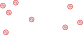
\includegraphics[width=0.75\textwidth]{pointset}
    \caption{Point Set for code walk-through.}
\end{figure}



\paragraph{Answer}

\todo{replace this TODO with your answer}
%%%%%%%%%%%%%%%%%%%%%%%%%%%%%%%%%%%%%%%%%%%%%%%%%%%%%%%%%%%%%%%%%%%%%%%%%%%%%%

%%%%%%%%%%%%%%%%%%%%%%%%%%%%%%%%%%%%%%%%%%%%%%%%%%%%%%%%%%%%%%%%%%%%%%%%%%%%%%
\collab{\todo{}}
\nextprob{Circle Intersection}

Assume you are given a collection of $n$ circles $\{C_1 , \ldots , C_n \}$ in
$\R^2$, where circle $C_i$ is presented as its center point $q_i = (x_i, y_i)$
and radius $r_i > 0$. Present a $\Theta(n \log n)$ time algorithm that determines
whether any two circles intersect. Note that one circle may be nested within
another without intersecting (see Figure 1). Your algorithm should either output
that there is no intersection, or that there is at least one intersection, and
if so it will output the indices of $i$ and $j$ of two circles $C_i$ and $C_j$
that intersect. Irrespective of the number of intersecting pairs, it need only
output one intersecting pair.

\begin{figure}[h]
    \centering
    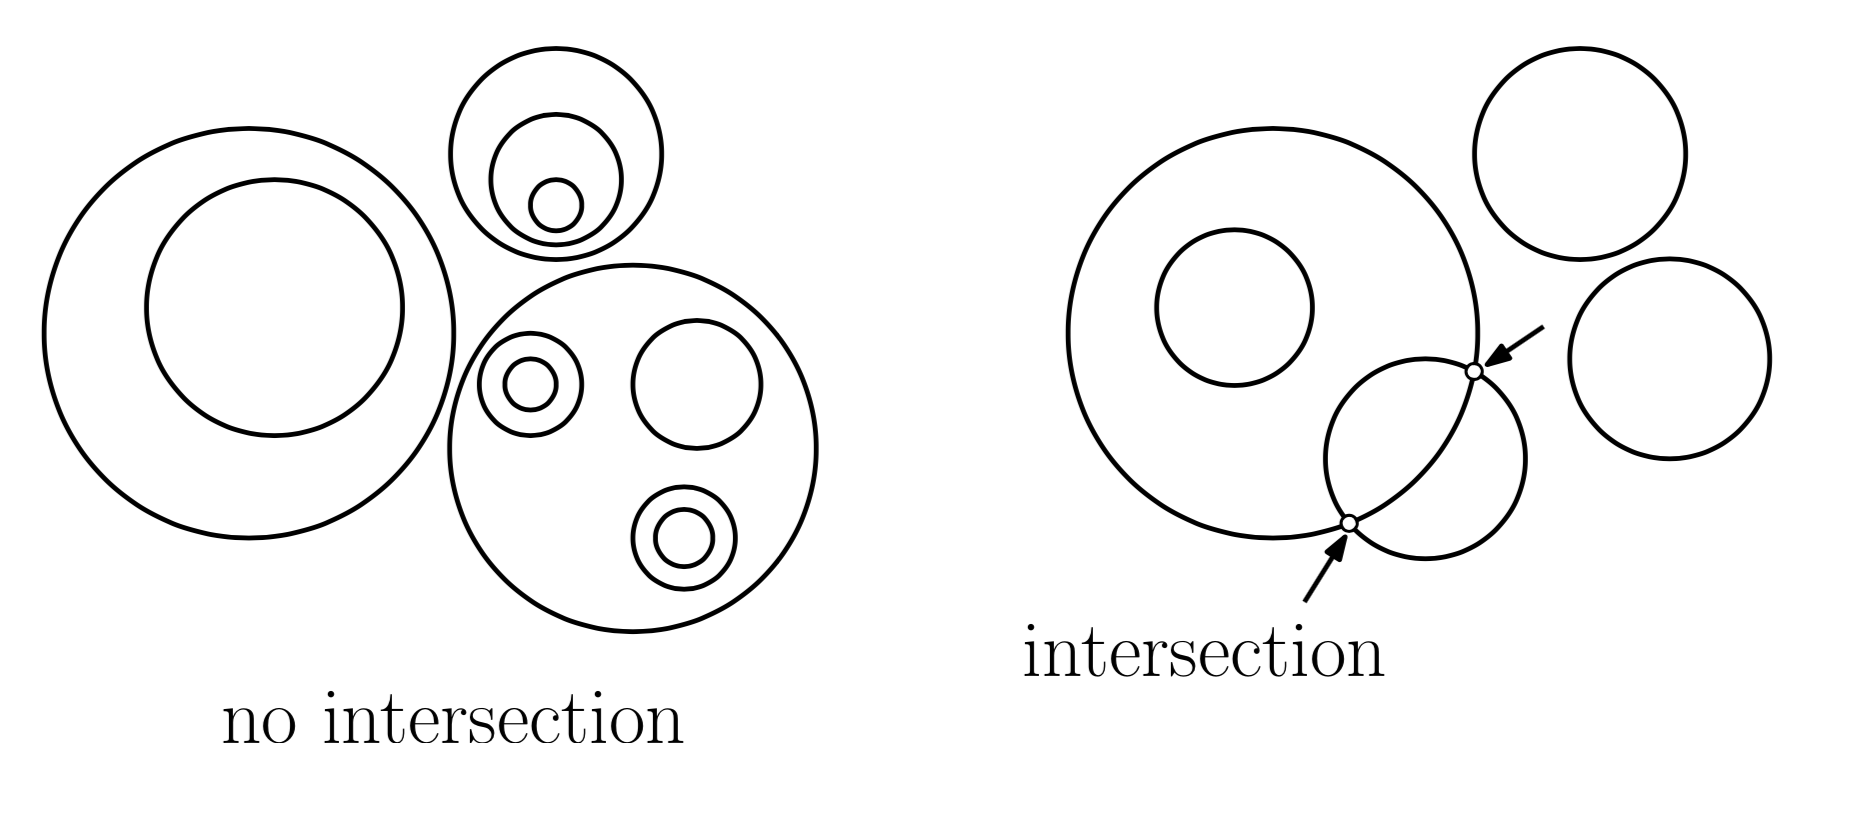
\includegraphics[width=0.75\textwidth]{intersection}
    \caption{Circle Intersection Example}
\end{figure}

Hint: Use plane-sweep. Explain clearly (1) what the sweep-line status stores and
what data structure is used to store this information and (2) what future events
are stored and what data structure is used. You may assume that you have access
to whatever primitive operations that you need in constant time. For example, if
you want to determine (a) whether two circles intersect, (b) the coordinates of
an intersection, (c) the intersection of a line with a circle, (d) whether a
point is contained within a circle's interior, etc., you may simply assume the
existence of a function that runs in $\Theta(1)$ time. As always, you may make
whatever general-position assumptions you like.

\paragraph{Answer}

\todo{replace this TODO with your answer}
%%%%%%%%%%%%%%%%%%%%%%%%%%%%%%%%%%%%%%%%%%%%%%%%%%%%%%%%%%%%%%%%%%%%%%%%%%%%%%

%%%%%%%%%%%%%%%%%%%%%%%%%%%%%%%%%%%%%%%%%%%%%%%%%%%%%%%%%%%%%%%%%%%%%%%%%%%%%%
\collab{\todo{}}
\nextprob{DCEL}

Assume you are given a planar subdivision of $\Theta(n)$ size in a DCEL. (You may
assume that the planar subdivision does not contain any holes, i.e., there are
no nested faces.) Describe an algorithm that for a given point $p$ in the plane
finds the face in the subdivision that contains it. Your algorithm should have
worst-case runtime of
$\Theta(n)$. You do not have to write pseudocode, but please make clear what
DCEL operations you are using. Also please make sure the analysis is detailed
enough to justify the $\Theta(n)$ runtime clearly.

\paragraph{Answer}

\todo{replace this TODO with your answer}
%%%%%%%%%%%%%%%%%%%%%%%%%%%%%%%%%%%%%%%%%%%%%%%%%%%%%%%%%%%%%%%%%%%%%%%%%%%%%%

%%%%%%%%%%%%%%%%%%%%%%%%%%%%%%%%%%%%%%%%%%%%%%%%%%%%%%%%%%%%%%%%%%%%%%%%%%%%%%
\collab{\todo{}}
\nextprob{Reflection}

Explain to me anything that you tried differently on this homework, focused on
for improvement of technical writing, or what you would especially like feedback
on.  It can be something simple like ``Before this class, I was not very aware
of what tense I was writing in.  For this homework, I tried to focus on writing
in present tense.'' or something very focused, such as ``I really focused on
improving my End-condition proofs for loop invariants.''  If you tried something
and struggled, let me know. Since everyone needs to improve (including me),
there should be something that you can write about here.  You can base it on
feedback I gave you, feedback I gave the class, feedback you received from
someone else, an example of technical writing that you really liked, or anything
else that motivates you to improve.

\paragraph{Answer}

\todo{replace this TODO with your answer}
%%%%%%%%%%%%%%%%%%%%%%%%%%%%%%%%%%%%%%%%%%%%%%%%%%%%%%%%%%%%%%%%%%%%%%%%%%%%%%

\end{document}
